\section*{Knuth-Morris-Pratt (KMP)}
\phantomsection
\addcontentsline{toc}{section}{Knuth-Morris-Pratt (KMP)}

\phantomsection
\subsection*{Introducción al Algoritmo de Knuth-Morris-Pratt}
% \addcontentsline{toc}{subsection}{Introducción al Algoritmo de Knuth-Morris-Pratt}
\quad Es un algoritmo que hace las comparaciones de izquierda a derecha, este realiza la búsqueda usando información basada en fallos previos obtenidos del patrón, esto se hace en una fase de “procesamiento” que crea una tabla de valores sobre su propio contenido. Esta tabla se crea para ver donde podría darse la siguiente coincidencia sin buscar más de 1 vez los caracteres del texto o cadena de caracteres donde se realiza la búsqueda, el algoritmo es de tiempo O~(n + m) siendo n = el tiempo de la fase de “searching” y m = el tiempo de la fase de procesamiento.
\\
\quad La tabla de fallos se encarga de evitar que cada carácter del texto sea analizado más de 1 vez, esto lo logra comparando el patrón consigo mismo para ver que partes se repiten. Este método guarda una lista con números le indican al algoritmo cuando debe devolverse desde la posición actual una vez que el patrón no coincida con el texto.

\quad El texto y el patrón van avanzando simultáneamente mientras ambos coincidan, si una vez coinciden del todo pero la letra siguiente sigue cumpliendo con el patrón, entonces el algoritmo mueve el patrón 1 a la derecha, si no coinciden, entonces el patrón se empieza a devolver para intentar hacerlo coincidir con el texto.

\phantomsection
\subsection*{Implementación del Algoritmo de Knuth-Morris-Pratt}
% \addcontentsline{toc}{subsection}{Implementación del Algoritmo de Knuth-Morris-Pratt}
(Con ayuda de \cite{KMP1}, \cite{KMPWiki} y \cite{KMPGFG})

\begin{algorithm} [H]
    \caption{Algoritmo de Knuth-Morris-Pratt}\label{alg:KMP}
    \begin{algorithmic} [1]
        \Procedure{knuth\_morris\_puth}{(texto, patron)}
            \State $n \gets \texttt{len(texto)}$
            \State $m \gets \texttt{len(patron)}$
            \State $resultado = False$
            \State $listaDeIndices = []$
            \State $tablaDeFallo = [0]*m$ \Comment{Tabla que se va a usar para devoluciones en los procesamientos}
            \State $i = 0$
            \State $j = 0$
            \Procedure{Procesamiento}{(patron, m, tablaDeFallo)}
                \State $longitud = 0$ \Comment{longitud del sufijo del prefijo mas largo}
                \State $i = 1$
                \While{$i < m$}
                    \If{$\texttt{patron[$i$]} == \texttt{patron[$longitud$]}$}
                        \State $longitud += 1$
                        \State $tablaDeFallo[i] = longitud$
                        \State $i += 1$
                    
                    \Else 
                        \If {$longitud != 0$} 
                            \State $longitud = tablaDeFallo[longitud-1]$
                        \Else
                            \State $tablaDeFallo[i] = 0$
                            \State $i += 1$
                        \EndIf
                    \EndIf
                \EndWhile
            \EndProcedure
            \Procedure{Búsqueda}{()}
                \State $i = 0$
                \State $j = 0$
                \While{$i < n$}
                    \If $patron[j] == texto[i]$
                        \State $i += 1$
                        \State $j += 1$
                        \EndIf
                        \If {$j == m$}
        \State $listaDeIndices += [i-j]$
        \State $resultado = True$
        \State $j = tablaDeFallo[j-1]$
        \ElsIf {$i < n \land patron[j] != text[i]$}
            \algstore{kmp}
    \end{algorithmic}
\end{algorithm}

\begin{algorithm} [H]
    \begin{algorithmic} [1]
    \algrestore{kmp}
        \If{$j != 0$}
            \State $j = tablaDeFallo[j-1]$
        \Else 
            \State $i += 1$
        \EndIf
    \EndIf
    \EndWhile
    \EndProcedure
    \State return listaDeIndices
    \EndProcedure
        
    \end{algorithmic}
\end{algorithm}



\subsection*{Análisis del Algoritmo de Knuth-Morris-Pratt}
% \addcontentsline{toc}{subsection}{Análisis del Algoritmo de Knuth-Morris-Pratt}
\subsubsection*{Paso 1: Establecer el tamaño n de los datos}
% \addcontentsline{toc}{subsubsection}{Paso 1: Establecer el tamaño n de los datos}
El tamaño esta dado por la cantidad de elementos en el texto * la cantidad de elementos en el patron
\[n = len(txt) * len(pat)\]


\subsubsection*{Paso 2: Determinar las operaciones de interés}
% \addcontentsline{toc}{subsubsection}{Paso 2: Determinar las operaciones de interés}
Comparaciones entre Pat y Txt y construcción de lps[] \\
    Suponemos el peor caso: todas son iguales a la mas grande de todas \\
    Asumimos que la mas grande vale 1 \\


\subsubsection*{Paso 3: Establecer la relacion de recurrencia para $\space T_{KMP}(n, m)$ con $\space n = len(txt) \land m = len(Pat)$}
% \addcontentsline{toc}{subsubsection}{Paso 3: Establecer la relacion de recurrencia para $\space T_{KMP}(n, m)$ con $\space n = len(txt) \land m = len(Pat)$}
Se obtuvo que: \[T_{KMP}(n, m) = m \hskip5cm                                   si n = 0\]
\[= (2 + t_{kmpS}(n-1)) + (1 + t_{kmpP}(m-1))\hskip1cm si n > 0\]
con kmpS = KMP search y kmpP = MKP Processing


\subsubsection*{Paso 4: Resolver la ecuacion de $T_{KMP}(n, m)$ eliminando la recursion}
% \addcontentsline{toc}{subsubsection}{Paso 4: Resolver la ecuacion de $T_{KMP}(n, m)$ eliminando la recursion}
\[T_{kmp}(n, m) = 2n + m\]

\subsubsection*{Paso 5: Determinar el orden de crecimiento asintotico de $T_{KMP}(n, m)$}
% \addcontentsline{toc}{subsubsection}{Paso 5: Determinar el orden de crecimiento asintotico de $T_{KMP}(n, m)$}
    \[T_{kmp}(n, m) \sim O(n + m)\]
    con n = el tiempo de la fase de “searching” y m = el tiempo de la fase de procesamiento.
\subsubsection*{Paso 6}
% \addcontentsline{toc}{subsubsection}{Paso 6}

\begin{figure} [H]
    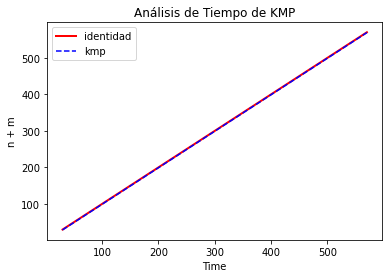
\includegraphics[width=0.5\textwidth]{../codigoPythonJupyter/kmp/Final.png}
    \caption{Knuth-Morris-Pratt (Apéndice kmp.ipynb)}
    \label{fig:kmp}
\end{figure}

%TODO
% https://discord.com/channels/965795707095232552/965795707736969320/990781609223540746
% https://discord.com/channels/965795707095232552/965795707736969320/987192403209388072

% https://discord.com/channels/965795707095232552/965795707736969320/987192403209388072

% https://discord.com/channels/965795707095232552/965795707736969320/987192403209388072